% checkpoint document for CIS581

\documentclass[10pt, twocolumn]{article}
\usepackage{graphicx}
\usepackage{color}
\usepackage{listings}
\usepackage{fullpage}
\usepackage{amsmath}
\usepackage{placeins}
\usepackage{caption}

%remove space at top of doc
\usepackage[showframe]{geometry}
\setlength{\voffset}{-1in}
\setlength{\headsep}{0pt}
\usepackage{titling}
\setlength{\droptitle}{-1cm}

\usepackage{subcaption}


\definecolor{lightgray}{gray}{0.5}
\setlength{\parindent}{0pt}
\setcounter{secnumdepth}{0} %turn off section numbering
\begin{document}

\title{CIS519 Final Project Checkpoint\vspace{-2ex}}
\author{Joe Trovato \and Justin Yim\vspace{-2ex}}
\date{10 December 2014\vspace{-2ex}}
\maketitle

\section{Option 2}
For this assignment Justin and I will be completing the second option specified in the homework. We plan to use code from previous projects and third party sources to produce a robust face replacement program. Most of the software we will be using can be found in the Matlab Vision Toolbox, but we are exploring other options as well. Our preliminary list of third party functions includes: vision.CascadeObjectDetector, corner, cornermetric, extractHOGFeatures, extractFeatures, and matchFeatures.

\section{Approach}
Our preliminary approach is outlined below. As the project progresses, we expect this to change to include elements of face replacement that we have not yet considered or run into. We predict these changes to occur to primarily in the (5) Refine Replacement Image step, in which there exist many possible implementations.\\
Our general approach is to follow this basic outline:
\begin{enumerate}
    \item Identify features in the replacement faces (3)
    \item Detect and extract faces in the source image (2)
    \item Identify features in the source faces (3)
    \item Match features in the source and replacement faces (3)
    \item Warp the source faces to the replacement face orientations (3)
    \item Select the closest matching source face to each replacement face (4)
    \item Color-correct the replacement face to match the source face (5)
    \item Create source and replacement face masks with blending (5)
    \item Replace source faces with the replacement faces (4)
We use Matlab's vision.CascadeObjectDetector for faces for step 2. We have explored two options for steps 1 and 3: HOG features, and face components. In the first approach, we detect corners with Matlab's corner function and extract HOG features which we match using matchFeatures. This approach produced very poor matches as shown. Our second approach uses matlab's eye, nose, and mouth detectors to find the bounding boxes of face components in each image. This approach produces a smaller number of control points (four in this case), but the detection is much more robust as seen below. This approach can be strengthened using a deformable part model.


\section{Preliminary Results} 
In our initial attempt at implementing the above algorithm we have achieve face detection, feature extraction per face, and are currently working on matching target faces to source faces. See figures below.

\begin{figure}[h!]
\centering
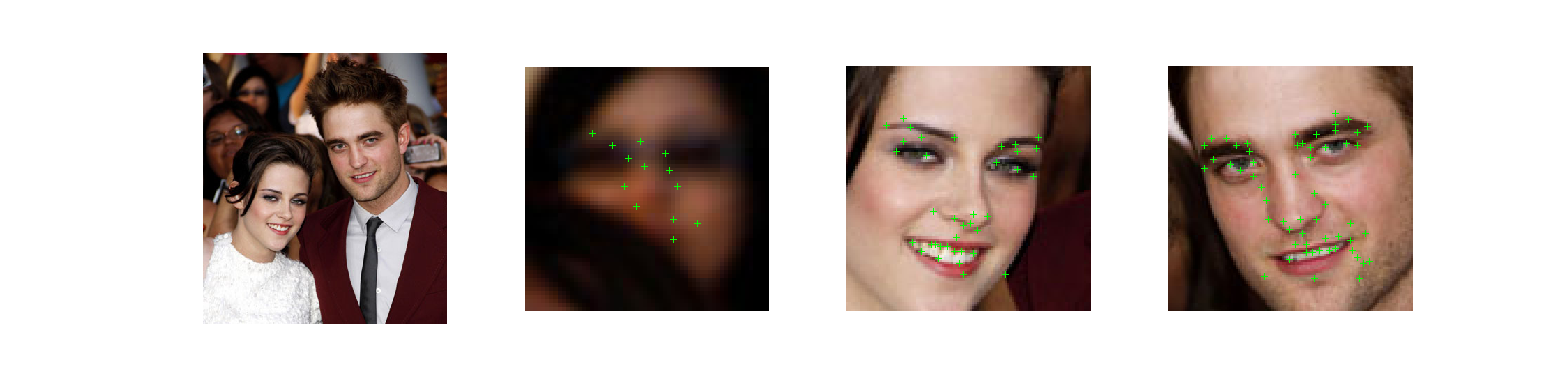
\includegraphics[width=0.7\linewidth]{figures/corner_detection.png}
\caption{corner detection on each face detected in the test image}
\end{figure}

\begin{figure}[h!]
\centering
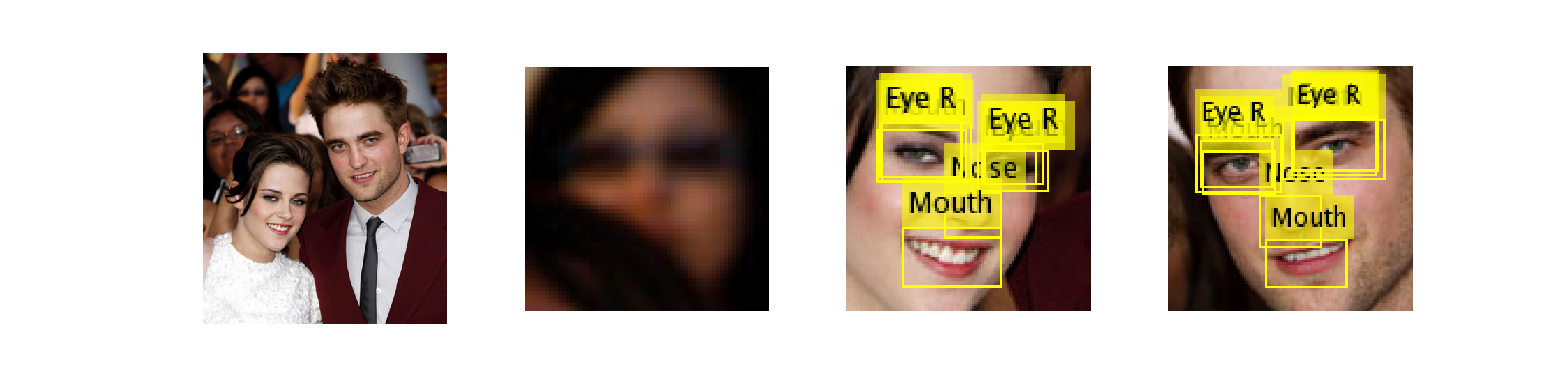
\includegraphics[width=0.7\linewidth]{figures/component_detection.png}
\caption{detecting face components on each face detected in the test image}
\end{figure}

\end{document}
